\documentclass[10pt,a4paper]{article}

\PassOptionsToPackage{hyphens}{url}
\usepackage[T1]{fontenc}
\usepackage{mathptmx}
\renewcommand{\ttdefault}{cmtt}
\usepackage[margin=0.68in]{geometry}
\usepackage{amsmath,amssymb}
\usepackage{graphicx}
\usepackage{booktabs}
\usepackage{tabularx}
\usepackage{multirow}
\usepackage{array}
\usepackage[dvipsnames,table]{xcolor}
\usepackage{enumitem}
\usepackage{caption}
\usepackage[colorlinks=true,linkcolor=NavyBlue,urlcolor=NavyBlue,citecolor=NavyBlue]{hyperref}

\setlength{\parskip}{3pt}
\setlength{\parindent}{0pt}
\emergencystretch=2em
\captionsetup{font=small,labelfont=bf}
\setlist[itemize]{leftmargin=1.35em,itemsep=1.5pt,topsep=1.5pt}

\definecolor{HdrBg}{HTML}{EAF2F8}
\definecolor{BoxBg}{HTML}{F7F9FB}

\newcommand{\meta}[4]{%
  \vspace{2pt}%
  \noindent\colorbox{BoxBg}{%
    \parbox{\dimexpr\textwidth-2\fboxsep\relax}{%
      \footnotesize\raggedright
      \textbf{File / Label:} \texttt{#1} \quad|\quad \textbf{Manuscript Location:} #2\\[1pt]
      \textbf{Generator / Source:} #3\\[1pt]
      \textbf{Primary Data Inputs:} #4%
    }%
  }\par\vspace{4pt}%
}

\begin{document}

% ============================================================================
% TITLE BLOCK
% ============================================================================
\begin{center}
  {\LARGE\bfseries Complete Guide to Generated Figures, Graphs, and Tables}\\[4pt]
  {\large Companion Reference for Paper 1 (14-Page Journal Manuscript):}\\[2pt]
  {\normalsize\itshape ``Who Backs Into the Bay? Benchmarking Information, Incentives, and Sim-to-3D Robustness in Narrow-Corridor Robot Negotiation''}\\[6pt]
  {\small Folder: \texttt{papers/paper1\_journal/} \quad|\quad Manuscript: \texttt{main.pdf} (14 pages) \quad|\quad Generator: \texttt{make\_figures.py}}
\end{center}
\vspace{2pt}
\hrule height 0.8pt
\vspace{6pt}

\noindent\textbf{Scope of This Document.}
This guide catalogs every visual artifact and quantitative summary table generated for the 14-page IEEE journal manuscript (\texttt{papers/paper1\_journal/main.pdf}). Specifically, it documents:
\begin{itemize}
  \item \textbf{7 multi-panel vector PDF figures comprising 20 individual sub-panels, graphs, and schematics} (\texttt{fig/*.pdf}), deterministically generated from raw per-episode CSVs and scenario configurations by \texttt{make\_figures.py}.
  \item \textbf{5 manuscript tables} (\texttt{Table I}--\texttt{Table V} in \texttt{papers/paper1\_journal/main.tex}), spanning policy taxonomy, the 18-study 2D + Gazebo experimental design ($50{,}374$ 2D episodes + $496$ Gazebo runs), the $2^3$ extreme-loss safeguard ablation, the seed-paired sim-to-3D transfer summary, and the practitioner selection matrix.
\end{itemize}
For every figure, individual sub-panel, and table, this guide explicitly states \textbf{(1) What It Shows} (axes, variables, baselines, sample sizes, uncertainty intervals, and visual encoding) and \textbf{(2) What It Means} (physical, algorithmic, or game-theoretic interpretation and key quantitative conclusions).

% ============================================================================
% SECTION 1: MASTER INVENTORY
% ============================================================================
\section{Master Inventory of Generated Figures and Tables}

\begin{table}[h!]\centering
\caption{Index of all 7 vector PDF figures (20 sub-panels) generated by \texttt{papers/paper1\_journal/make\_figures.py}.}
\footnotesize\setlength{\tabcolsep}{3.6pt}
\begin{tabularx}{\textwidth}{@{}lllc>{\raggedright\arraybackslash}Xl@{}}\toprule
\rowcolor{HdrBg}\textbf{Fig.} & \textbf{PDF File} & \textbf{Generator} & \textbf{Panels} & \textbf{Graphs / Sub-Panels Included} & \textbf{Sec. / Page} \\\midrule
Fig.~1 & \texttt{fig/scenarios.pdf} & \texttt{fig1\_scenarios} & 6 & (a) Single-bay map; (b) Two-bay map; (c) Convoy 2v1 map; (d) T-junction map; (e) Gazebo Harmonic 3D Waffle frame; (f) Waffle clearance cross-section & Sec.~III-A, p.~4 \\
Fig.~2 & \texttt{fig/protocol.pdf} & \texttt{fig2\_protocol} & 2 & (a) 20\,Hz 5-mode agent state machine \& safeguards; (b) Snapshot exchange \& constant-speed kinematic yield timeline & Sec.~III-C, p.~4 \\
Fig.~3 & \texttt{fig/rq1\_information.pdf} & \texttt{fig3\_rq1\_information} & 4 & (a) Single-bay geometry \& FCFS reservation (\texttt{S1}); (b) Asymmetric urgency/load/speed (\texttt{S2}); (c) Log-normal bid-noise sweep (\texttt{S7}); (d) Tabular bandit ID vs.\ OOD layout shift & Sec.~VI, p.~9 \\
Fig.~4 & \texttt{fig/rq2\_incentives.pdf} & \texttt{fig4\_rq2\_incentives} & 2 & (a) Misreport utility gain curves across payment rules (\texttt{S9}); (b) Repeated-encounter delay vs.\ Jain fairness Pareto (\texttt{S10}) & Sec.~VII, p.~10 \\
Fig.~5 & \texttt{fig/rq3\_comms\_maps.pdf} & \texttt{fig5\_rq3\_comms\_maps} & 2 & (a) Packet-loss \& latency scaling up to 99\% (\texttt{S3}+\texttt{S8b}); (b) Online bay discovery \& map-sharing excess (\texttt{explore}) & Sec.~VIII, p.~11 \\
Fig.~6 & \texttt{fig/rq4\_topologies.pdf} & \texttt{fig6\_rq4\_topologies} & 2 & (a) Convoy 2-vs.-1 weighted delay with \texttt{make\_room}; (b) 3-robot T-junction completion \& delay before/after \texttt{goal\_wait} & Sec.~IX-A, p.~12 \\
Fig.~7 & \texttt{fig/rq4\_gazebo.pdf} & \texttt{fig7\_rq4\_gazebo} & 2 & (a) 460-run seed-paired Gazebo-vs.-2D delay scatter; (b) Seed-3 spacetime trace $x(t)$ showing Gazebo lidar-clustering lag & Sec.~IX-B, p.~13 \\\bottomrule
\end{tabularx}
\\[2pt]{\scriptsize Total across Figs.~1--7: $6 + 2 + 4 + 2 + 2 + 2 + 2 = 20$ individual panels ($8$ geometric maps/frames/diagrams + $12$ quantitative empirical plots).}
\end{table}

\begin{table}[h!]\centering
\caption{Index of all 5 manuscript tables authored in \texttt{papers/paper1\_journal/main.tex}.}
\footnotesize\setlength{\tabcolsep}{4pt}
\begin{tabularx}{\textwidth}{@{}llc>{\raggedright\arraybackslash}Xl@{}}\toprule
\rowcolor{HdrBg}\textbf{Table} & \textbf{LaTeX Label} & \textbf{Size} & \textbf{Summary Scope \& Underlying Source Data} & \textbf{Sec. / Page} \\\midrule
Table~I & \texttt{tab:taxonomy} & $9\times 7$ & Architectural taxonomy of all 9 policies (\texttt{R, S, F, D, P, L, C, G, V}) across comms, inputs, motion model, and incentives (\texttt{policy.py}, \texttt{planner.py}, \texttt{agent.py}) & Sec.~IV, p.~6 \\
Table~II & \texttt{tab:design} & $19\times 6$ & Complete factorial experimental matrix covering 18 2D studies ($50{,}374$ episodes) + ROS~2 / Gazebo validation ($460+36$ runs) grouped by RQ1--RQ4 & Sec.~V-B, p.~8 \\
Table~III & \texttt{tab:abl} & $8\times 7$ & Condensed $2^3$ extreme-loss safeguard ablation (\texttt{S8c}, $5{,}760$ episodes at 90--99\% loss, 2--8\,s latency) from \texttt{S8c\_protocol\_ablation.csv.gz} & Sec.~VIII-A, p.~10 \\
Table~IV & \texttt{tab:gz} & $16\times 6$ & Seed-paired ROS~2 Jazzy / Gazebo Harmonic transfer results across 14 main scenario groups ($460$ runs) + 2 Batch-2 groups ($36$ runs) & Sec.~IX-B, p.~11 \\
Table~V & \texttt{tab:guide} & $5\times 4$ & Practitioner policy and protocol selection matrix mapping 5 warehouse deployment regimes to recommended policies, flags, and quantitative trade-offs & Sec.~X-A, p.~12 \\\bottomrule
\end{tabularx}
\end{table}

\clearpage
% ============================================================================
% SECTION 2: DETAILED GUIDE TO ALL 7 GENERATED FIGURES
% ============================================================================
\section{Detailed Guide to Generated Figures and Sub-Panel Graphs}

% ----------------------------------------------------------------------------
% FIGURE 1
% ----------------------------------------------------------------------------
\subsection{Figure 1: Physical Problem Setup, Topologies, and Clearance Geometry}

\meta{fig/scenarios.pdf (label: fig:scenarios)}{Section III-A, Page 4}{\texttt{make\_figures.py :: fig1\_scenarios()}}{\texttt{configs/scenarios/corridor\_single\_bay.yaml}, \texttt{corridor\_two\_bays.yaml}, \texttt{corridor\_convoy.yaml}, \texttt{corridor\_tjunction\_goal.yaml}, and \texttt{media/gazebo\_final/corridor\_cost\_bid.webp}}

\begin{center}
  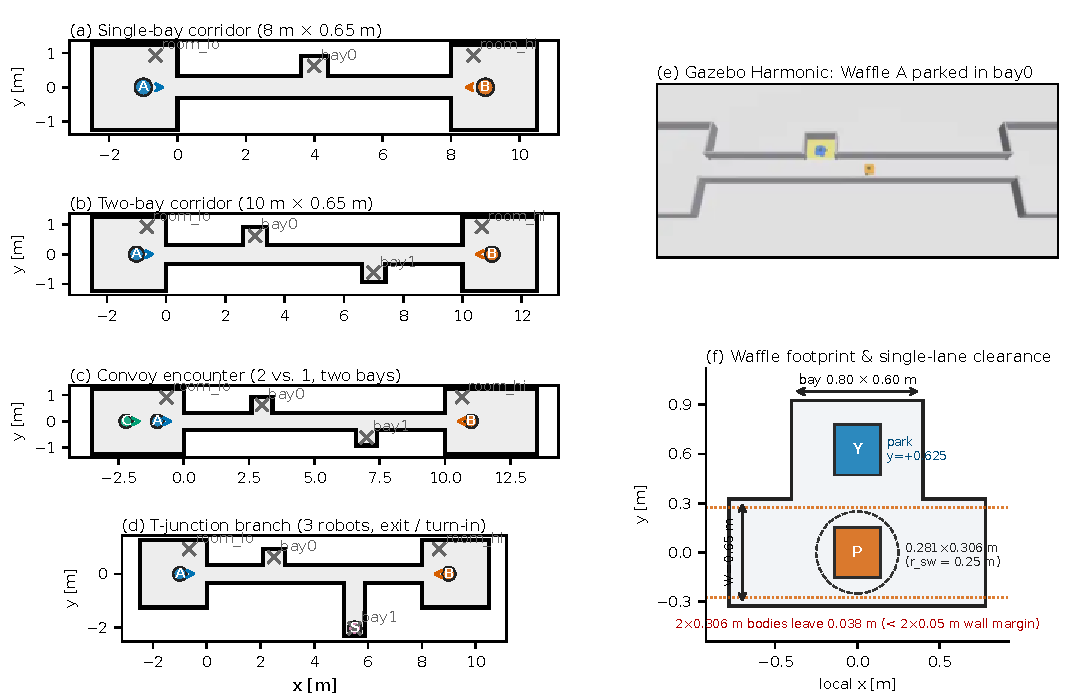
\includegraphics[width=0.80\textwidth]{fig/scenarios.pdf}
\end{center}

\textbf{Panel-by-Panel Breakdown:}
\begin{itemize}
  \item \textbf{Panels (a)--(d) --- Benchmark Corridor Topologies:}
  \begin{itemize}
    \item \emph{What They Show:} Four 2D metric floorplans ($x$ vs.\ $y$ in meters) rendered directly from the scenario YAML files used by both simulators, showing corridor walls, Staging Rooms (\texttt{room\_lo} at $x<0$, \texttt{room\_hi} at $x>L$), lateral pull-in refuge bays ($0.80\times 0.60$\,m), and initial robot poses/headings: (a) single-bay straight corridor ($8.0\times 0.65$\,m) with opposing robots $A$ (blue) and $B$ (orange); (b) two-bay corridor ($10.0\times 0.65$\,m) with opposing bays at $x=3$\,m and $x=7$\,m; (c) 2-vs.-1 convoy encounter where follower $C$ (green) trails leader $A$ against oncoming $B$; and (d) 3-robot T-junction where a $2.0$\,m deep side branch at $x=7$\,m (\texttt{bay1}) hosts robot $S$ (purple) while $A$ and $B$ contest the main aisle and upstream \texttt{bay0} ($x=3$\,m).
    \item \emph{What They Mean:} Establish the progressive topological complexity of the benchmark---moving from an isolated binary choice of \emph{who} yields in a single-bay aisle (a), to \emph{where} and \emph{with what map knowledge} to yield in multi-bay aisles (b), to coupled multi-robot chain reactions where pairwise negotiation alone deadlocks without follower \texttt{make\_room} (c) or upstream \texttt{goal\_wait} (d).
  \end{itemize}
  \item \textbf{Panel (e) --- ROS~2 Jazzy / Gazebo Harmonic 3D Execution Frame:}
  \begin{itemize}
    \item \emph{What It Shows:} An overhead snapshot extracted from an actual Gazebo Harmonic run (frame 48 of \texttt{corridor\_\allowbreak cost\_bid.webp}), depicting TurtleBot3 Waffle $A$ parked off-lane inside \texttt{bay0} while Waffle $B$ passes unimpeded along the $y=0$ corridor centerline.
    \item \emph{What It Means:} Demonstrates visually that the exact same 20\,Hz negotiation state machine executes on full 3D rigid-body differential-drive models with simulated $360^\circ$ GPU ray-cast lidar and extruded wall geometry.
  \end{itemize}
  \item \textbf{Panel (f) --- Waffle Chassis Footprint and Single-Lane Clearance Cross-Section:}
  \begin{itemize}
    \item \emph{What It Shows:} Exact metric cross-section of the $W=0.65$\,m aisle and $0.80\times 0.60$\,m pull-in bay, plotting the rectangular TurtleBot3 Waffle chassis ($0.281\times 0.306$\,m), its $R_{\mathrm{sw}}=0.25$\,m turn-in-place swept circle, the $0.05$\,m safety wall margins (orange dotted lines), Proceeder $P$ centered at $y=0$, and Yielder $Y$ parked at $y_{\mathrm{park}}=+0.625$\,m.
    \item \emph{What It Means:} Proves geometrically \emph{why continuous local collision avoidance (e.g., ORCA/CBF) cannot solve this problem without discrete bay negotiation}: two $0.306$\,m-wide Waffle bodies side-by-side consume $0.612$\,m inside a $0.650$\,m corridor, leaving only $0.038$\,m total clearance---violating the required $2\times 0.05 = 0.10$\,m wall margin and making lateral passing physically impossible anywhere outside a refuge bay.
  \end{itemize}
\end{itemize}

\clearpage
% ----------------------------------------------------------------------------
% FIGURE 2
% ----------------------------------------------------------------------------
\subsection{Figure 2: Simulator-Agnostic Protocol State Machine and Kinematic Yield Timeline}

\meta{fig/protocol.pdf (label: fig:proto)}{Sections III-C \& IV-B, Page 4}{\texttt{make\_figures.py :: fig2\_protocol()}}{Architectural specification of \texttt{amr\_negotiation/agent.py} and \texttt{amr\_negotiation/planner.py} (Eqs.~1--2)}

\begin{center}
  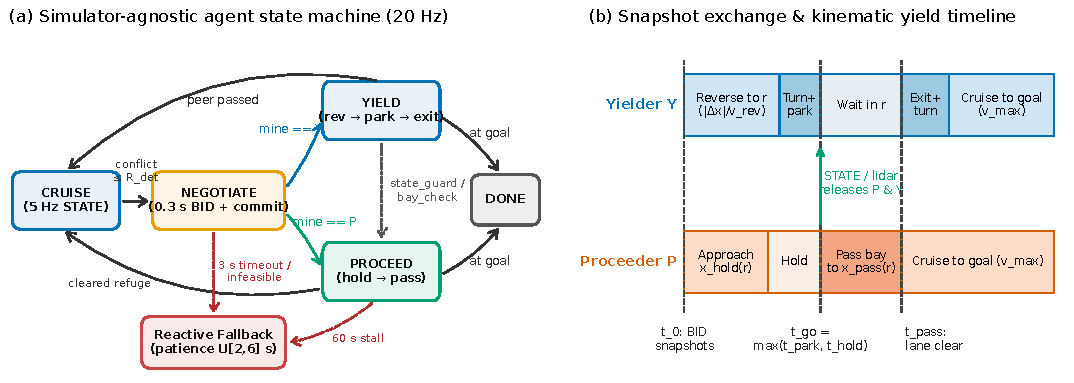
\includegraphics[width=0.95\textwidth]{fig/protocol.pdf}
\end{center}

\textbf{Panel-by-Panel Breakdown:}
\begin{itemize}
  \item \textbf{Panel (a) --- Simulator-Agnostic 20\,Hz Agent State Machine:}
  \begin{itemize}
    \item \emph{What It Shows:} A directed finite-state machine diagram depicting the five primary control modes (\texttt{CRUISE} with $5$\,Hz \texttt{STATE} beacons, \texttt{NEGOTIATE} with $0.3$\,s \texttt{BID} broadcasts and optional \texttt{commit} confirmation, \texttt{YIELD} executing reverse $\to$ turn $\to$ park $\to$ exit, \texttt{PROCEED} executing approach $\to$ hold $\to$ pass, and \texttt{DONE}), alongside the \texttt{Reactive Fallback} mode (random patience $U[2,6]$\,s) triggered on $3$\,s negotiation timeout, infeasible refuge sets, or $60$\,s stall timeouts, plus the cross-transitions for \texttt{state\_guard} and \texttt{bay\_check}.
    \item \emph{What It Means:} Clarifies the strict architectural separation between \textbf{Layer 2 (Protocol \& Execution)}, which handles asynchronous message drops, timeouts, and physical safety guards identically across all policies, and \textbf{Layer 1 (Decision Mechanism)}, which plugs into \texttt{NEGOTIATE} purely to map frozen snapshots $(S_A,S_B)$ to $(Y, r)$. It also makes explicit the exact safeguard edges later ablated in Table~III (\texttt{S8c}).
  \end{itemize}
  \item \textbf{Panel (b) --- Snapshot Exchange and Constant-Speed Kinematic Yield Timeline:}
  \begin{itemize}
    \item \emph{What It Shows:} A synchronized two-track horizontal timeline comparing Yielder $Y$'s five motion phases (reverse $|x_r-x_Y|/v_{\mathrm{rev}}$, $90^\circ$ turn + park into $y_{\mathrm{park}}$, wait in refuge $r$, exit + turn, and cruise at $v_{\max}$) against Proceeder $P$'s four motion phases (approach $x_{\mathrm{hold}}(r)$, hold if $Y$ is not yet parked, pass bay to $x_{\mathrm{pass}}(r)$, and cruise to goal), anchored by synchronization instants $t_0$ (\texttt{BID} snapshot freeze), $t_{\mathrm{go}}=\max(t_{\mathrm{park}}, t_{\mathrm{hold}})$, and $t_{\mathrm{pass}}$ (lane clear release via \texttt{STATE} or lidar).
    \item \emph{What It Means:} Visually explains Equations~(1)--(2) of the paper: why yielding delay is non-linear in bay position (reversing uses slower $v_{\mathrm{rev}}=0.18$\,m/s plus two $90^\circ$ turns and lateral bay entry/exit, while $P$ only waits $\max(0, t_{\mathrm{park}}-t_{\mathrm{hold}})$), and how \texttt{cost\_bid} and \texttt{clarke} price candidate outcomes in sub-millisecond CPU time without forward physics rollouts.
  \end{itemize}
\end{itemize}

\clearpage
% ----------------------------------------------------------------------------
% FIGURE 3
% ----------------------------------------------------------------------------
\subsection{Figure 3: RQ1 --- Information Fidelity, Geometry, Bid Noise, and Layout Shift}

\meta{fig/rq1\_information.pdf (label: fig:rq1)}{Section VI (RQ1), Page 9}{\texttt{make\_figures.py :: fig3\_rq1\_information()}}{\texttt{data/raw/classical/S1\_baseline.csv.gz}, \texttt{reservation.csv.gz}, \texttt{S2\_asymmetry.csv.gz}, \texttt{S7\_noisy\_bids.csv.gz}, and \texttt{data/tables/classical/learned\_negotiator.md}}

\begin{center}
  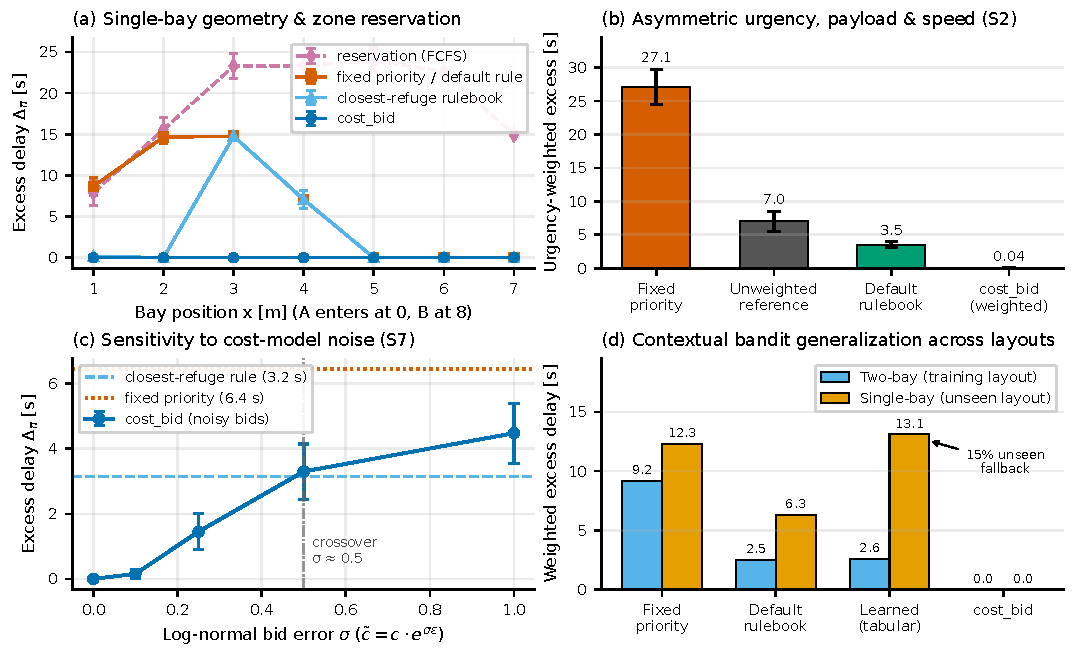
\includegraphics[width=0.66\textwidth]{fig/rq1_information.pdf}
\end{center}

{\small
\textbf{Panel-by-Panel Breakdown:}
\begin{itemize}
  \item \textbf{Panel (a) --- Single-Bay Geometry Sweep and Zone Reservation (\texttt{S1} + \texttt{reservation}):}
  \begin{itemize}
    \item \emph{What It Shows:} Mean paired excess delay $\Delta_\pi = D_\pi - \min(D_A,D_B)$ [s] ($\pm 95\%$ CI) on the $y$-axis plotted against single-bay position $x\in\{1,2,3,4,5,6,7\}$\,m on the $x$-axis ($A$ enters at $x=0$, delayed $B$ at $x=8$\,m), comparing FCFS corridor \texttt{reservation} ($N=1{,}260$, purple diamonds), \texttt{fixed\_priority}/\texttt{rules\_default} ($N=2{,}940$, orange squares), \texttt{rules\_proximity} (sky-blue triangles), and \texttt{cost\_bid} (blue circles).
    \item \emph{What It Means:} Demonstrates three core RQ1 findings: (1) industrial FCFS corridor locking (\texttt{reservation}) wastes $18.8\pm 0.9$\,s excess delay across all bay positions because holding outside the aisle requires turning off-lane in \texttt{room\_hi} and forfeits mid-corridor bays entirely; (2) static ID priority and seniority-first rulebooks suffer severe $14.6$--$14.8$\,s spikes at $x=2$--$3$\,m by forcing $B$ to reverse nearly the whole corridor even when $A$ just passed a bay; and (3) promoting geometric proximity (\texttt{rules\_proximity}) halves excess delay to $3.1$\,s, while kinematic \texttt{cost\_bid} achieves $\Delta_\pi = 0.0$\,s at every bay coordinate ($100\%$ hindsight-optimal yielder match).
  \end{itemize}
  \item \textbf{Panel (b) --- Heterogeneous Robot Urgency, Payload, and Speed (\texttt{S2}, $N=5{,}040$):}
  \begin{itemize}
    \item \emph{What It Shows:} Bar chart with 95\% CI error bars comparing urgency-weighted excess delay [s] against the weighted hindsight reference (\texttt{oracle\_w}) across four policies on asymmetric encounters ($u_B\in\{1,3\}$, payload $\{0,1\}$, $v_B\in\{0.26,0.13\}$\,m/s): \texttt{fixed\_priority} ($27.1$\,s), unweighted hindsight \texttt{oracle} ($7.0$\,s), \texttt{rules\_default} ($3.5$\,s), and weighted \texttt{cost\_bid} ($0.04$\,s).
    \item \emph{What It Means:} Proves that \emph{objective alignment matters more than kinematic precision}: even an omniscient oracle optimizing unweighted time loses $7.0$\,s of urgency-weighted delay---twice the $3.5$\,s excess of a simple 6-rule etiquette (\texttt{rules\_default}) that respects urgency and payload. Weighted \texttt{cost\_bid} captures virtually the entire remaining gap ($0.04\pm 0.02$\,s, matching \texttt{oracle\_w} on $704/720 = 98\%$ of encounters).
  \end{itemize}
  \item \textbf{Panel (c) --- Sensitivity to Multiplicative Bid-Estimation Noise (\texttt{S7}, $N=3{,}150$):}
  \begin{itemize}
    \item \emph{What It Shows:} Excess delay $\Delta_\pi$ [s] ($\pm 95\%$ CI) of \texttt{cost\_bid} plotted against log-normal multiplicative bid noise standard deviation $\sigma\in\{0, 0.1, 0.25, 0.5, 1.0\}$ ($\tilde{c}=c\cdot e^{\sigma\epsilon}$), benchmarked against horizontal reference lines for noise-free \texttt{rules\_proximity} ($3.2$\,s) and \texttt{fixed\_priority} ($6.4$\,s), with the crossover marked at $\sigma\approx 0.5$.
    \item \emph{What It Means:} Pinpoints the exact model-fidelity threshold required for auction-based coordination: \texttt{cost\_bid} strictly dominates heuristic rulebooks when travel-time estimation error is $\sigma\le 0.25$ ($\Delta_\pi \le 1.5$\,s), reaches statistical parity with the closest-refuge rulebook at $\sigma=0.5$ ($\sim 1.65\times$ multiplicative error, $3.3$\,s vs.\ $3.2$\,s), and degrades below the rulebook for $\sigma > 0.5$ while still beating static ID priority even at $\sigma=1.0$ ($4.5$\,s vs.\ $6.4$\,s).
  \end{itemize}
  \item \textbf{Panel (d) --- Tabular Contextual Bandit Generalization Across Corridor Layouts (\texttt{learned}):}
  \begin{itemize}
    \item \emph{What It Shows:} Grouped bar chart comparing weighted excess delay [s] on the held-out \emph{training} two-bay layout (light blue bars, $n=150$) vs.\ an \emph{unseen} single-bay layout with random bay coordinates (gold bars, $n=150$) across \texttt{fixed\_priority}, \texttt{rules\_default}, \texttt{learned} (trained offline on 800 forced two-bay pairs, 93 populated state keys), and \texttt{cost\_bid}.
    \item \emph{What It Means:} Shows that while a model-free tabular bandit easily matches the engineered rulebook in-distribution ($+2.6$\,s vs.\ $+2.5$\,s), it suffers severe out-of-distribution failure under layout shift ($+13.1$\,s, worse than fixed priority's $+12.3$\,s, with $15\%$ unseen-key fallbacks). Coarse ego-centric feature bins memorize layout-specific bay priors rather than transferable stopping-distance physics.
  \end{itemize}
\end{itemize}
}

\clearpage
% ----------------------------------------------------------------------------
% FIGURE 4
% ----------------------------------------------------------------------------
\subsection{Figure 4: RQ2 --- Strategic Misreporting Incentives and Repeated Fairness}

\meta{fig/rq2\_incentives.pdf (label: fig:rq2)}{Section VII (RQ2), Page 10}{\texttt{make\_figures.py :: fig4\_rq2\_incentives()}}{\texttt{data/raw/classical/S9\_payments.csv.gz} ($10{,}080$ eps) and \texttt{data/raw/classical/S10\_repeated.csv.gz} ($50\times 20$ encounters)}

\begin{center}
  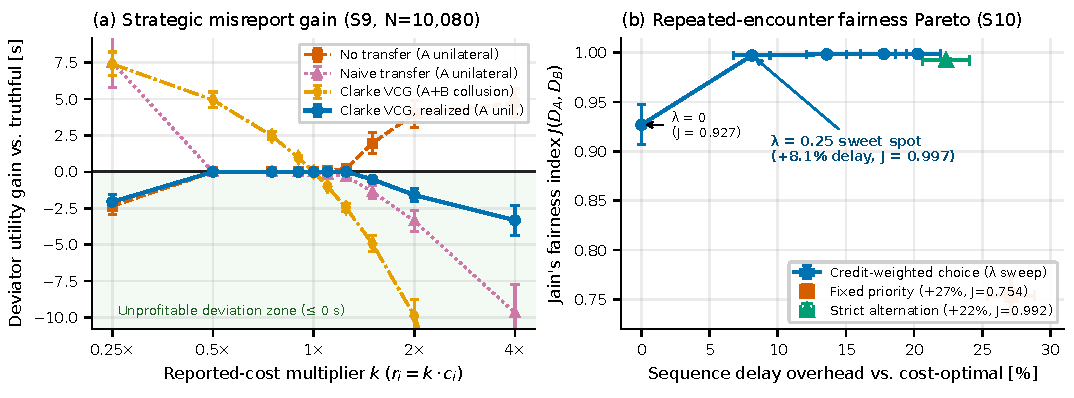
\includegraphics[width=0.95\textwidth]{fig/rq2_incentives.pdf}
\end{center}

\textbf{Panel-by-Panel Breakdown:}
\begin{itemize}
  \item \textbf{Panel (a) --- Single-Encounter Strategic Misreport Gain Across Payment Mechanisms (\texttt{S9}, $N=10{,}080$):}
  \begin{itemize}
    \item \emph{What It Shows:} Mean deviator quasi-linear utility gain [s] relative to truthful bidding ($k=1\times$) ($\pm 95\%$ CI) on the $y$-axis vs.\ logarithmic report-scaling multiplier $k\in[0.25\times, 4\times]$ ($r_i = k\cdot c_i$) on the $x$-axis. The green shaded region ($\le 0$\,s) denotes unprofitable lies. Four mechanisms/coalitions are plotted: unpriced \texttt{cost\_bid} unilateral $A$ (orange dashed squares), naive ``proceeder-pays-yielder's-bid'' transfer unilateral $A$ (purple dotted triangles), joint $A+B$ collusion under Clarke VCG (gold dash-dotted diamonds), and realized-trajectory unilateral $A$ under Clarke VCG (solid blue circles).
    \item \emph{What It Means:} Proves empirically both the power and boundaries of VCG mechanism design in physical robotics: (1) unpriced \texttt{cost\_bid} rewards bid inflation ($+4.74$\,s gain at $k=4\times$ by forcing the peer to yield); (2) naive direct transfers backfire by rewarding bid \emph{under-reporting} ($+7.54$\,s gain at $k=0.25\times$); (3) Clarke pivot payments completely eliminate unilateral misreport gains ($0.00$\,s predicted; $\le +0.02\pm 0.02$\,s on realized simulator trajectories, bending downward to $-3.3$\,s at extreme $k$); yet (4) joint $A+B$ bid shading ($k<1$) beats the external bank ($+4.94$\,s combined gain at $0.5\times$, $+7.42$\,s at $0.25\times$) because scaling both bids down preserves the allocation while shrinking both pivot charges.
  \end{itemize}
  \item \textbf{Panel (b) --- Repeated-Encounter Efficiency vs.\ Cumulative Fairness Pareto Frontier (\texttt{S10}):}
  \begin{itemize}
    \item \emph{What It Shows:} A 2D trade-off scatter/curve over 50 random 20-encounter sequences (with horizontal and vertical 95\% CI bars), plotting percentage sequence delay overhead above pure cost-optimal selection ($\lambda=0$) on the $x$-axis against Jain's cumulative fairness index $J(D_A^{\mathrm{cum}}, D_B^{\mathrm{cum}})\in[0.5,1.0]$ on the $y$-axis. Compares the cumulative-delay credit sweep $\lambda\in\{0, 0.25, 0.5, 1.0, 2.0\}$ (Eq.~6, blue curve) against \texttt{fixed\_priority} (orange square) and strict turn-taking \texttt{alternate} (green triangle).
    \item \emph{What It Means:} Shows that in cooperative single-owner fleets, VCG transfers are unnecessary to achieve long-run equity: static \texttt{fixed\_priority} is both unfair ($J=0.754$) and slow ($+27.1\%$ overhead), while strict alternation reaches $J=0.992$ only by wasting $+22.3\%$ delay when bays are asymmetric. A lightweight non-monetary fairness weight of $\lambda=0.25$ hits a sharp Pareto sweet spot---achieving near-perfect cumulative equity ($J=0.997$) for just $+8.1\%$ delay overhead by flipping only close-call encounters toward the historically burdened robot.
  \end{itemize}
\end{itemize}

\clearpage
% ----------------------------------------------------------------------------
% FIGURE 5
% ----------------------------------------------------------------------------
\subsection{Figure 5: RQ3 --- Channel Impairment Resilience and Online Map Sharing}

\meta{fig/rq3\_comms\_maps.pdf (label: fig:rq3)}{Section VIII (RQ3), Page 11}{\texttt{make\_figures.py :: fig5\_rq3\_comms\_maps()}}{\texttt{data/raw/classical/S3\_comms.csv.gz}, \texttt{S8b\_comms\_extreme.csv.gz}, and \texttt{explore\_map.csv.gz}}

\begin{center}
  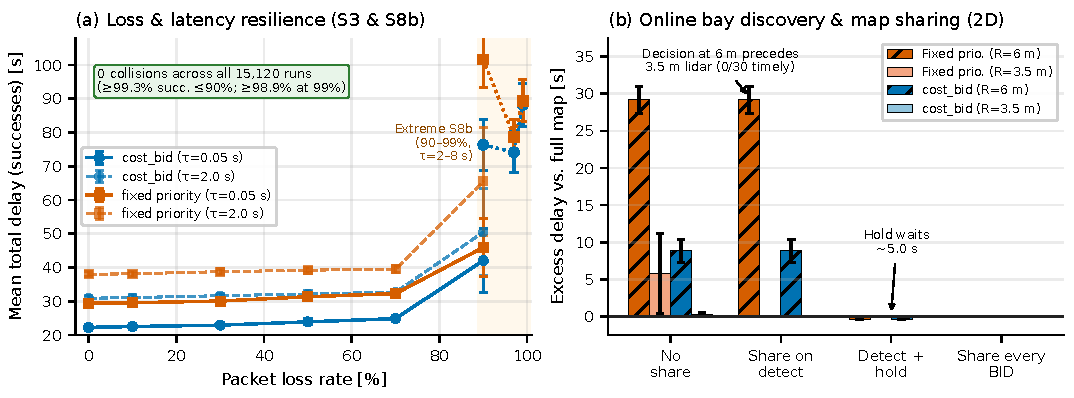
\includegraphics[width=0.95\textwidth]{fig/rq3_comms_maps.pdf}
\end{center}

\textbf{Panel-by-Panel Breakdown:}
\begin{itemize}
  \item \textbf{Panel (a) --- Packet Loss and Latency Scaling Up to 99\% Loss (\texttt{S3} + Extreme \texttt{S8b}):}
  \begin{itemize}
    \item \emph{What It Shows:} Mean total delay over successful episodes [s] ($\pm 95\%$ CI) vs.\ Bernoulli packet drop rate from $0\%$ to $99\%$, plotting \texttt{cost\_bid} (blue circles) and \texttt{fixed\_priority} (orange squares) at base latencies $\tau=0.05$\,s (solid) and $\tau=2.0$\,s (dashed) from \texttt{S3} ($v_{\max}=0.26$\,m/s, $3{,}600$ eps), seamlessly joined on the right (amber shaded band, $90$--$99\%$ loss) by extreme stress study \texttt{S8b} ($\tau=2$--$8$\,s, $v_{\max}=0.50$\,m/s, $1{,}440$ eps).
    \item \emph{What It Means:} Demonstrates remarkable protocol grace under harsh industrial Wi-Fi degradation: across all $15{,}120$ communication and ablation runs (\texttt{S3}+\texttt{S8}+\texttt{S8b}+\texttt{S8c}), \textbf{zero collisions occurred}, with completion $\ge 99.3\%$ up to $90\%$ loss and $98.9$--$99.2\%$ at $99\%$ loss. Periodic $0.3$\,s \texttt{BID} broadcasts keep delay completely flat ($<2$\,s rise) up to $50\%$ packet loss, and \texttt{cost\_bid} preserves its $\sim 8$--$10$\,s delay advantage over \texttt{fixed\_priority} across every loss and latency tier.
  \end{itemize}
  \item \textbf{Panel (b) --- Online Bay Discovery and Map-Sharing Modes in 2D (\texttt{explore}, $0\%$ Loss):}
  \begin{itemize}
    \item \emph{What It Shows:} Grouped bar chart ($\pm 95\%$ CI) of paired excess delay [s] relative to full prior map knowledge across four map-sharing configurations---\texttt{No share}, \texttt{Share on detect}, \texttt{Detect + hold} (\texttt{hold\_for\_map}), and \texttt{Share every BID}---comparing \texttt{fixed\_priority} and \texttt{cost\_bid} at conflict detection ranges $R_{\mathrm{det}}=6.0$\,m (hatched) vs.\ $R_{\mathrm{det}}=3.5$\,m (solid) ($1{,}800$-episode \texttt{explore\_map} dataset).
    \item \emph{What It Means:} Reveals a critical cross-layer timing trap between radio negotiation range and onboard sensor range: at default $R_{\mathrm{det}}=6.0$\,m, robots freeze snapshots and commit to a yield plan \emph{before} their $3.5$\,m lidars ever detect each other ($0/30$ timely maps), making \texttt{share\_on\_detect} just as costly as never sharing maps ($+29.2$\,s for \texttt{fixed\_priority}, $+8.8$\,s for \texttt{cost\_bid}). While \texttt{hold\_for\_map} or shrinking $R_{\mathrm{det}}$ to $3.5$\,m fixes this in 2D ($\approx 0$\,s excess), unconditionally piggybacking known bay IDs on every \texttt{BID} (\texttt{Share every BID}) achieves $+0.0$\,s excess immediately at $6.0$\,m with zero holding delay.
  \end{itemize}
\end{itemize}

\clearpage
% ----------------------------------------------------------------------------
% FIGURE 6
% ----------------------------------------------------------------------------
\subsection{Figure 6: RQ4a --- Multi-Robot Convoys and T-Junction Topologies}

\meta{fig/rq4\_topologies.pdf (label: fig:rq4\_topo)}{Section IX-A (RQ4), Page 12}{\texttt{make\_figures.py :: fig6\_rq4\_topologies()}}{\texttt{data/raw/classical/convoy\_group.csv.gz} ($1{,}080$ eps), \texttt{tjunction\_goal.csv.gz} ($384$ eps), and \texttt{data/tables/classical/tjunction\_goal\_before.txt}}

\begin{center}
  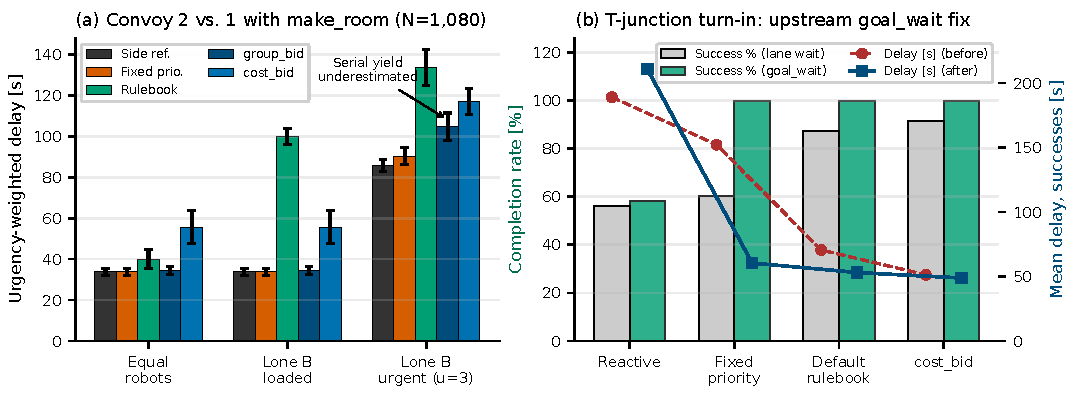
\includegraphics[width=0.95\textwidth]{fig/rq4_topologies.pdf}
\end{center}

\textbf{Panel-by-Panel Breakdown:}
\begin{itemize}
  \item \textbf{Panel (a) --- Two-vs.-One Convoy Encounters with Follower \texttt{make\_room} ($N=1{,}080$):}
  \begin{itemize}
    \item \emph{What It Shows:} Grouped bar chart ($\pm 95\%$ CI) of urgency-weighted delay [s] across three opponent regimes---\texttt{Equal robots} ($u=1$), \texttt{Lone B loaded}, and \texttt{Lone B urgent} ($u_B=3$)---comparing hindsight \texttt{side\_oracle} (charcoal), \texttt{fixed\_priority} (orange), \texttt{rules\_default} (green), side-level \texttt{group\_bid} (dark blue), and pairwise \texttt{cost\_bid} (medium blue), with follower \texttt{make\_room} enabled ($72/72$ completion in every cell).
    \item \emph{What It Means:} Shows both the necessity and the modeling subtlety of group-level bidding: at equal urgency, pairwise \texttt{cost\_bid} prices only leader $A$ and ignores follower $C$ ($55.6$\,s), whereas \texttt{group\_bid} prices the whole convoy and slashes delay to $34.4$\,s (matching \texttt{side\_oracle}'s $33.7$\,s). However, when lone $B$ has $u_B=3$, \texttt{group\_bid} ($104.7$\,s) beats pairwise \texttt{cost\_bid} ($117.1$\,s) yet trails \texttt{fixed\_priority} ($90.3$\,s) and \texttt{side\_oracle} ($85.7$\,s) because Eq.~(4) sums member delays additively rather than modeling the \emph{serial} wait while follower $C$ backs out of leader $A$'s reversal path.
  \end{itemize}
  \item \textbf{Panel (b) --- Three-Robot T-Junction Turn-In Before vs.\ After Upstream \texttt{goal\_wait}:}
  \begin{itemize}
    \item \emph{What It Shows:} Dual-axis chart ($0\%$ loss, $n=48$ episodes per policy) comparing episode completion rate [\%] on the left axis (gray bars = before fix, holding in main lane; green bars = after adding upstream bay staging \texttt{goal\_wait}) and mean successful-episode delay [s] on the right axis (red dashed circles = before; dark-blue solid squares = after) across \texttt{reactive}, \texttt{fixed\_priority}, \texttt{rules\_default}, and \texttt{cost\_bid}.
    \item \emph{What It Means:} Demonstrates that three-robot branch junctions induce coupled gridlock when a robot whose branch goal (\texttt{bay1}) is occupied waits in the main stem while an oncoming robot approaches. Adding the topological \texttt{goal\_wait} rule (parking temporarily in upstream \texttt{bay0} until \texttt{bay1} clears) lifts negotiating-policy completion from $60.4\%\text{--}91.7\%$ to \textbf{100\% ($48/48$)} across all three negotiating policies while cutting \texttt{fixed\_priority} delay from $152.2$\,s to $60.5$\,s and achieving $48.9\pm 4.0$\,s under \texttt{cost\_bid}.
  \end{itemize}
\end{itemize}

\clearpage
% ----------------------------------------------------------------------------
% FIGURE 7
% ----------------------------------------------------------------------------
\subsection{Figure 7: RQ4b --- 496-Run ROS~2 / Gazebo Transfer and Lidar-Lag Trace}

\meta{fig/rq4\_gazebo.pdf (label: fig:rq4\_gz)}{Section IX-B (RQ4), Page 13}{\texttt{make\_figures.py :: fig7\_rq4\_gazebo()}}{\texttt{data/tables/gazebo/gazebo\_main\_runs.csv}, \texttt{gazebo\_all\_runs.csv}, \texttt{media/gazebo\_final/explore\_det35\_fixed\_priority.json}, \texttt{explore\_all35\_fixed\_priority.json}, and \texttt{sim2d}}

\begin{center}
  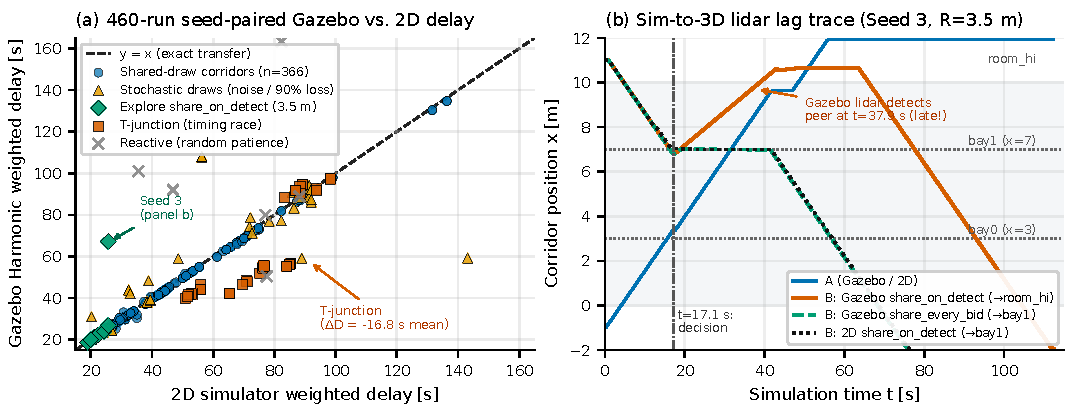
\includegraphics[width=0.95\textwidth]{fig/rq4_gazebo.pdf}
\end{center}

\textbf{Panel-by-Panel Breakdown:}
\begin{itemize}
  \item \textbf{Panel (a) --- 460-Run Seed-Paired Gazebo Harmonic vs.\ 2D Weighted Delay Scatter:}
  \begin{itemize}
    \item \emph{What It Shows:} Per-episode scatter plot of Gazebo urgency-weighted delay [s] ($y$-axis) against identical-seed 2D simulator weighted delay [s] ($x$-axis) across all paired successful episodes in the 460-run main grid, stratified by regime relative to the $y=x$ exact-transfer diagonal: 366 shared-draw straight/convoy corridor runs (blue circles), independent stochastic draws under bid noise or 90\% loss (gold triangles), $3.5$\,m \texttt{explore share\_on\_detect} runs (green diamonds), 36 T-junction runs (orange squares), and \texttt{reactive} random-patience runs (gray crosses).
    \item \emph{What It Means:} Visually separates where fast 2D kinematic benchmarking is sufficient from where 3D physics-in-the-loop simulation is mandatory: all 366 shared-draw corridor runs cluster tightly along $y=x$ (policy-level excess delays agree within $\le 1.0$\,s and yielder choices match in $96.8\%$ of negotiating runs), whereas systematic off-diagonal clusters pinpoint two genuine sim-to-3D transfer gaps---Gazebo lidar peer-clustering lag (green diamonds above $y=x$, including annotated Seed~3) and three-robot T-junction stem-release timing races (orange squares below $y=x$, $\Delta D=-16.8$\,s mean).
  \end{itemize}
  \item \textbf{Panel (b) --- Empirical Sim-to-3D Spacetime Trajectory $x(t)$ on Seed 3 ($R_{\mathrm{det}}=3.5$\,m):}
  \begin{itemize}
    \item \emph{What It Shows:} Longitudinal corridor position $x(t)\in[-2,12]$\,m vs.\ simulation time $t\in[0,115]$\,s for Seed~3 under \texttt{fixed\_priority} in \texttt{explore} mode ($R_{\mathrm{det}}=3.5$\,m), marking \texttt{bay0} ($x=3$\,m), \texttt{bay1} ($x=7$\,m), and \texttt{room\_hi} ($x>10$\,m). Compares Robot $A$'s trajectory (solid blue) against three paired trajectories for yielding Robot $B$: Gazebo \texttt{share\_on\_detect} (solid orange, reversing all the way to \texttt{room\_hi}), Gazebo \texttt{share\_every\_bid} (dashed green, ducking into \texttt{bay1}), and 2D \texttt{share\_on\_detect} (dotted black, also ducking into \texttt{bay1}).
    \item \emph{What It Means:} Provides the exact physical mechanism behind the \texttt{explore} sim-to-3D discrepancy: in 2D, idealized range check detects peer $A$ inside $3.5$\,m before the $t=17.1$\,s decision freeze so $A$ shares \texttt{bay1} in time; in 3D Gazebo, wall-filtered \texttt{LaserScan} clustering (\texttt{cluster\_dist} $0.35$\,m) does not register oncoming Waffle $A$'s small front profile until $2.3$--$2.6$\,m separation (occurring late at $t=37.9$\,s after $B$ has already reversed to \texttt{room\_hi}), costing $\sim 41$\,s of unnecessary reversing on Seed~3. Unconditional \texttt{share\_map} on every \texttt{BID} completely eliminates this 3D sensor-clustering bottleneck.
  \end{itemize}
\end{itemize}

\clearpage
% ============================================================================
% SECTION 3: DETAILED GUIDE TO ALL 5 MANUSCRIPT TABLES
% ============================================================================
\section{Detailed Guide to All 5 Manuscript Tables}

% ----------------------------------------------------------------------------
% TABLE I
% ----------------------------------------------------------------------------
\subsection{Table I: Taxonomy of Benchmarked Corridor Coordination Policies}

\meta{Table I (label: tab:taxonomy)}{Section IV, Page 6}{Authored in \texttt{papers/paper1\_journal/main.tex} (lines 139--156)}{Synthesizes exact implementation properties of \texttt{amr\_negotiation/policy.py}, \texttt{planner.py}, and \texttt{agent.py}}

\begin{itemize}
  \item \textbf{What It Shows:} A 9-row $\times$ 7-column architectural comparison of every policy evaluated in the paper---\texttt{reactive} (R), \texttt{reservation} (S), \texttt{fixed\_priority} (F), \texttt{rules\_default} (D), \texttt{rules\_proximity} (P), \texttt{learned} (L), \texttt{cost\_bid} (C), \texttt{group\_bid} (G), and \texttt{clarke} (V)---classified across \emph{Family}, \emph{Comms Required} (None, \texttt{STATE} only, or \texttt{STATE}+\texttt{BID}), \emph{State Inputs Used}, \emph{Motion Model} (None, Feasibility only, Refuge distance, Offline sim table, Constant-speed, or Side-level sum), \emph{Strategic Incentive Property}, and \emph{Multi-Robot / Map Scope}, with explicit footnotes clarifying non-bid attack surfaces and VCG budget-surplus/collusion caveats.
  \item \textbf{What It Means:} Gives readers a unified conceptual ladder ordered by increasing information and modeling fidelity---showing that all negotiating policies share the exact same radio packet format and execution layer, differing solely in how much physical state, kinematic modeling, and game-theoretic pricing they apply to select $(Y, r)$.
\end{itemize}

% ----------------------------------------------------------------------------
% TABLE II
% ----------------------------------------------------------------------------
\subsection{Table II: Complete Factorial Experimental Design Matrix}

\meta{Table II (label: tab:design)}{Section V-B, Page 8}{Authored in \texttt{papers/paper1\_journal/main.tex} (lines 247--277)}{\texttt{experiments/classical/*.py}, \texttt{data/raw/classical/*.csv.gz}, and \texttt{experiments/gazebo/make\_scen\_all.py}}

\begin{itemize}
  \item \textbf{What It Shows:} A 19-row $\times$ 6-column master experimental table organized into four horizontal blocks matching \textbf{RQ1} (6 studies: \texttt{S1}, \texttt{reservation}, \texttt{S4}, \texttt{S2}, \texttt{S7}, \texttt{learned}), \textbf{RQ2} (3 studies: \texttt{S6}, \texttt{S9}, \texttt{S10}), \textbf{RQ3} (7 studies: \texttt{S3}, \texttt{S8}, \texttt{S8b}, \texttt{S8c}, Asymmetric maps, Blocked bays, Explore \& hold), and \textbf{RQ4} (3 studies: Convoy 2v1, 3-robot T-junction, and ROS~2 / Gazebo 3D). For each study, it lists exact factorial grid parameters, random seed counts ($2$--$60$), evaluated policy codes, and exact episode counts $N$ ($50{,}374$ 2D episodes + $460+36=496$ Gazebo episodes).
  \item \textbf{What It Means:} Establishes full statistical transparency and reproducibility across the entire study suite, making immediately clear which studies share identical episode draws (enabling tight paired excess-delay confidence intervals) and how the 496 Gazebo runs stratify across every 2D study family.
\end{itemize}

% ----------------------------------------------------------------------------
% TABLE III
% ----------------------------------------------------------------------------
\subsection{Table III: Extreme-Loss Factorial Safeguard Ablation}

\meta{Table III (label: tab:abl)}{Section VIII-A (RQ3), Page 10}{Authored in \texttt{papers/paper1\_journal/main.tex} (lines 344--362)}{\texttt{data/raw/classical/S8c\_protocol\_ablation.csv.gz} ($5{,}760$ episodes; verified via \texttt{data/tables/classical/round2\_studies.md})}

\begin{itemize}
  \item \textbf{What It Shows:} Reports the $2^3$ full-factorial ablation of protocol safeguards (\texttt{commit} $\in\{\text{on, off}\} \times \texttt{state\_guard} \in\{\text{on, off}\} \times \texttt{bay\_check} \in\{\text{on, off}\}$) for \texttt{fixed\_priority} and \texttt{cost\_bid} across the worst-case \texttt{S8b} channel grid ($90$--$99\%$ packet loss, $2$--$8$\,s latency, $v_{\max}=0.5$\,m/s; 360 episodes per row, condensed to 8 distinct rows because \texttt{bay\_check} had zero triggers and identical episode-by-episode metrics). Columns report \emph{Success \%}, \emph{Deadlock count}, \emph{Mean Delay $\pm$ 95\% CI [s]}, and \emph{Transient Dual-Yield \%}, noting \textbf{0 collisions in every arm} (95\% upper bound $1.06\%$).
  \item \textbf{What It Means:} Delivers a crucial negative engineering result: under $90$--$99\%$ packet loss and multi-second latency, radio-based confirmation handshakes (\texttt{commit}) and stale beacon guards (\texttt{state\_guard}) are \emph{not} what prevent physical collisions---local lidar stopping margins and randomized $U[6,12]$\,s park-release timers carry safety even when all three radio guards are turned off. Worse, enabling \texttt{commit} under extreme loss adds $+3.1$--$3.8$\,s delay and \emph{increases} transient dual-yield starts ($15$--$16\% \to 22$--$24\%$) by holding robots undecided until the $3.0$\,s timeout triggers simultaneous reactive fallbacks.
\end{itemize}

\clearpage
% ----------------------------------------------------------------------------
% TABLE IV
% ----------------------------------------------------------------------------
\subsection{Table IV: 496-Run Seed-Paired ROS~2 / Gazebo Harmonic Transfer Summary}

\meta{Table IV (label: tab:gz)}{Section IX-B (RQ4), Page 11}{Authored in \texttt{papers/paper1\_journal/main.tex} (lines 387--411)}{\texttt{data/tables/gazebo/gazebo\_all.md}, \texttt{gazebo\_main\_runs.csv}, \texttt{gazebo\_all\_runs.csv}, and \texttt{reports/gazebo/hold\_for\_map\_results.md}}

\begin{itemize}
  \item \textbf{What It Shows:} A 16-row $\times$ 6-column breakdown of all $460$ main Gazebo validation runs (14 scenario/study groups covering \texttt{S1}, \texttt{reactive}, forced yielders, \texttt{S2}, \texttt{S4}, \texttt{S7}, \texttt{S9}, \texttt{S3}, \texttt{S8b/c}, Convoy, T-junction, Asymmetric maps, Blocked bays, and Explore) plus the $36$ Batch-2 runs (\texttt{hold\_for\_map} and \texttt{det\_3.5} rerun). Columns report \emph{Runs}, \emph{Successes}, \emph{Collisions}, \emph{Same First Yielder count} vs.\ paired 2D seed, and \emph{Mean Delay Offset $\Delta D = D_{\mathrm{Gz}} - D_{\mathrm{2D}}$ [s]}.
  \item \textbf{What It Means:} Quantifies exact sim-to-3D transfer fidelity across the entire benchmark:
  \begin{enumerate}[leftmargin=1.6em,itemsep=1pt,topsep=1pt]
    \item \emph{Zero-collision safety:} $486/486$ non-reactive Gazebo episodes succeeded with $0$ collisions ($0.85\%$ 95\% upper bound on the 450 main runs), whereas uncoordinated \texttt{reactive} suffered $1$ collision in $10$ Gazebo runs.
    \item \emph{Sub-second straight-corridor fidelity:} $393/406$ ($96.8\%$) negotiating episodes chose the exact same yielder as 2D, and deterministic straight/convoy groups exhibit $|\Delta D| \le 1.2$\,s.
    \item \emph{Pinpointed 3D divergences:} Large $|\Delta D|$ values isolate purely to T-junction stem-release races ($\Delta D = -16.8$\,s) and \texttt{hold\_for\_map} lidar-clustering delay ($\Delta D = +10.0$\,s), telling practitioners exactly which multi-robot/sensor interactions require 3D testing.
  \end{enumerate}
\end{itemize}

% ----------------------------------------------------------------------------
% TABLE V
% ----------------------------------------------------------------------------
\subsection{Table V: Practitioner Policy and Protocol Selection Matrix}

\meta{Table V (label: tab:guide)}{Section X-A (Discussion), Page 12}{Authored in \texttt{papers/paper1\_journal/main.tex} (lines 413--425)}{Distills quantitative decision rules across RQ1--RQ4 ($>50{,}000$ 2D + $496$ Gazebo episodes)}

\begin{itemize}
  \item \textbf{What It Shows:} A 5-row $\times$ 4-column engineering decision table mapping five concrete warehouse deployment regimes---(1) homogeneous cooperative fleet with uncertain kinematics ($\sigma\ge 0.5$); (2) heterogeneous urgent, loaded, and mixed-speed cooperative fleet ($\sigma\le 0.25$); (3) self-interested / multi-vendor shared aisles; (4) multi-robot convoys and T-junction branches; and (5) legacy bay-less aisles with off-lane staging---to \emph{Recommended Policy}, \emph{Protocol Configuration Flags}, and \emph{Empirical Basis \& Caveats}.
  \item \textbf{What It Means:} Translates the paper's 18 experimental studies into immediately actionable architecture guidelines: rather than claiming a single policy wins everywhere, it specifies exact quantitative thresholds ($\sigma=0.5$ noise crossover, $\lambda=0.25$ fairness credit, unconditional \texttt{share\_map} over \texttt{share\_on\_detect}, Clarke VCG only when multi-vendor incentives outweigh $29$--$44\%$ bank surplus, and mandatory \texttt{make\_room} and \texttt{goal\_wait} rules for $\ge 3$-robot topologies).
\end{itemize}

\end{document}
